
\subsection{Cluster expansion}

A Hamiltonian of the folowing form is assumed
\begin{equation}
    \hat{H}_n = \sum_{i=1}^{n-1} \hat{h} _{i,i+1}+ \sum_{i=1}^n \hat{h'}_i
\end{equation}
Virtual level zero is defined as follows:
\begin{equation}
    \begin{split}
        \mpo{1}{ {0,0}  }{}{}{}{} &=  \expH{1}{}{{,,,,,,,,}}{{,,,,,,,,}}{}
    \end{split}
\end{equation}
Similarly, the contraction of elements $O_{01}$ and $O_{10}$ are defined as follows:
\begin{equation}
    \mpo{2}{{0,1,0}}{}{}{}{} =  \expH{2}{}{}{}{} - \mpo{2}{{0,,0}}{}{}{}{}
\end{equation}
Some notation will be introduced that will be used later on. The rensor $L_n$ is the contraction of n MPO's where the virtual index increases between each bond. $R_n$ is similar but the virtual bond starts from n and decreases. The tensor is defined in gra[hical notation by:

\def \On {\mpo{4}{ {0,1,,"m","n"}  }{}{}{{0,0,1,0,0}}{}}
\def \OnBlock {\expH{4}{ $L_n$  }{ {,,"...",} }{ {,,"...",} }{{0,"n"}} }

\begin{equation}
    \begin{split}
        &\OnBlock = \On\\
    \end{split}
\end{equation}

\def \MnBlock {\expH{4}{ $M_n$  }{ {,,"...",} }{ {,,"...",} }{}{} }
\def \expHBlock {\expH{4}{ $e^{- \beta \hat{H}_{n}}$   }{ {,,"...",} }{ {,,"...",} }{}{} }
\def \Mn {\mpo{4}{ {0,,,,0}  }{}{}{{0,0,1,0,0}}{}}

\noindent $M_n$ is the difference between the exponentiated hamiltonian for n sites and the contraction of the MPO over all the currently assigned combinations of virtual levels.

\begin{equation}
    \begin{split}
        \MnBlock &=  \expHBlock \\
        &-\Mn \\
    \end{split}
\end{equation}

In what follows different constructions will detailed. Some notes on the practical implementation is given later in this section.

\subsubsection{Type A}
This type was originally proposed in \cite{Vanhecke2021}. The following types of blocks appear in the cluster expansion:

\mpo{1}{ {"n","m"}  }{}{}{}{},\mpo{1}{ {"m ","n"}  }{}{}{}{} and \mpo{1}{ {"n","n"}  }{}{}{}{} with $n \in \mathbb{N}_0$ and $m=n-1$.

\paragraph{$O^{n n}$}

The $O^{n n}$ block is defined by \cref{eq_nn_level}

\def \rhs{\expH{1}{ $L_{n}^{-1}  M_{2n+1}  R_{n}^{-1}$ }{}{}{{"n","n"}}  }

\begin{equation}
    \mpo{1}{ {"n","n"}  }{}{}{}{} = \rhs
    \label{eq_nn_level}
\end{equation}
The residual error M is calculated for a chain of size $2n+1$. The left and right inverses $L_n$ and $R_n$ are applied to M to find the block $O^{n n}$.

\paragraph{ $O^{m n }$ and $O^{n m} $}
The contraction of $O^{n m }$ and $O^{m n} $ is defined by:

\def \rhs{\expH{2}{ $L_{n}^{-1}  M_{2n+2}  R_{n}^{-1}$ }{}{}{{"n","n"}}  }
\begin{equation}
    \mpo{2}{ {"n","m","n"}  }{}{}{}{} = \rhs
    \label{eq_nmn_level2}
\end{equation}

The individual elements $O^{m n }$ and $O^{n m} $ are obtained by doing an svd decoposition as explained in \cref{decompMPO}. The square root of the singuar values is multiplied to the left and right of the decomposition. The operator $L_{n+1}$ and $R_{n+1}$ can be construdted directly. \todo{implementeren en testen.}

During the svd the bond dimension can be lowered by only keeping the rows and colums belonging to $\sigma_i > \sigma_0$. This also helps the invertibility. Increasing $\sigma_0$ reduces the precision of the MPO.

\paragraph{Truncation}

Intoduction of a new block can result in large fluctuating errors. This happens because the inverses are possible ill conditioned. Therefore the construction of the MPO should be stopped at a certain optimal order. Many different criteria can be tought of (and have been tried), but the most reliable method is as follows:

\paragraph{ \( O^{n n} \)}

The \( O^{n n} \) blocks can form long chains. To test whether these chains improve accuracy, the norm (see \cref{mponormdef}) of the residul error is calculated before and after the insertion of the block for a cyclic chain. A closed chain is used with the same number of sites. The closed chain resembles much better an infite chain than the open counterpart.

Only strict improvements are accepted, otherwise the MPO without the newly calculated blocks is returned.

\paragraph{$O^{m n}$ and $O^{n m}$ } For these the same procedure holds.

\paragraph{dimension}

From the construction is can be seen that  the dimension of the new virtual level is at most $d^2$ times the dimension of the previous level. Depending on $\sigma_0$, the bond dimension is even lower.

\paragraph{discussion}

The only parameter in the construction is $\sigma_0$ As can be seen in \cref{fig:sigman0}, mainly the construction for small values of $\beta$ get affected by the choice of $\sigma_0$.This can be seen in \cref{fig:sigman0}. A good tradeoff seems to be $ \sigma_0 = {10}^{-12}$. There is almost no precision loss vor small $\beta$, while for intermediate it performs optimal for intermediate $\beta$.

\begin{figure}
    \centering
    \begin{subfigure}{\textwidth}
        \centering
        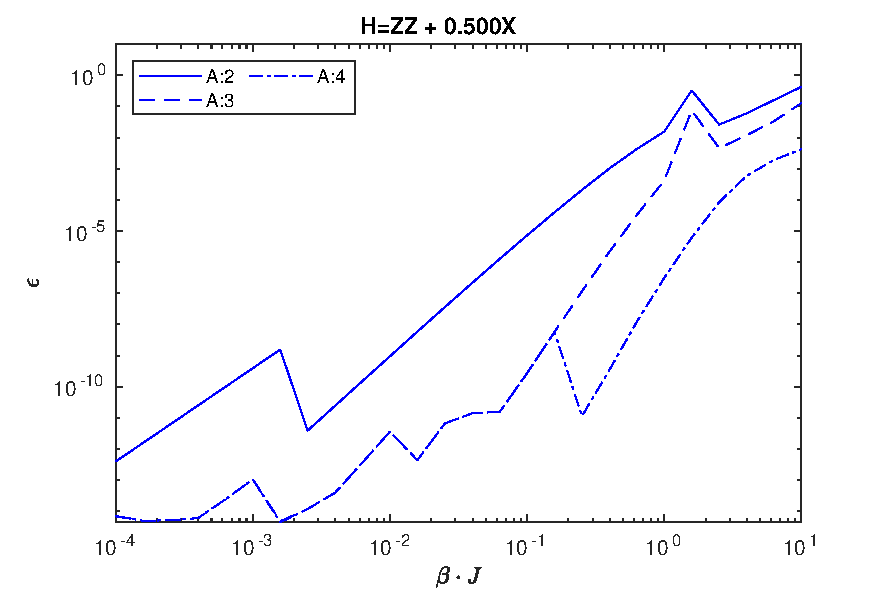
\includegraphics[width=0.8\linewidth]{Figuren/mpo_construction/sigm0/e10.pdf}
        \caption{ ${10}^{-10}$}
        \label{fig:sub1}
    \end{subfigure}%

    \begin{subfigure}{\textwidth}
        \centering
        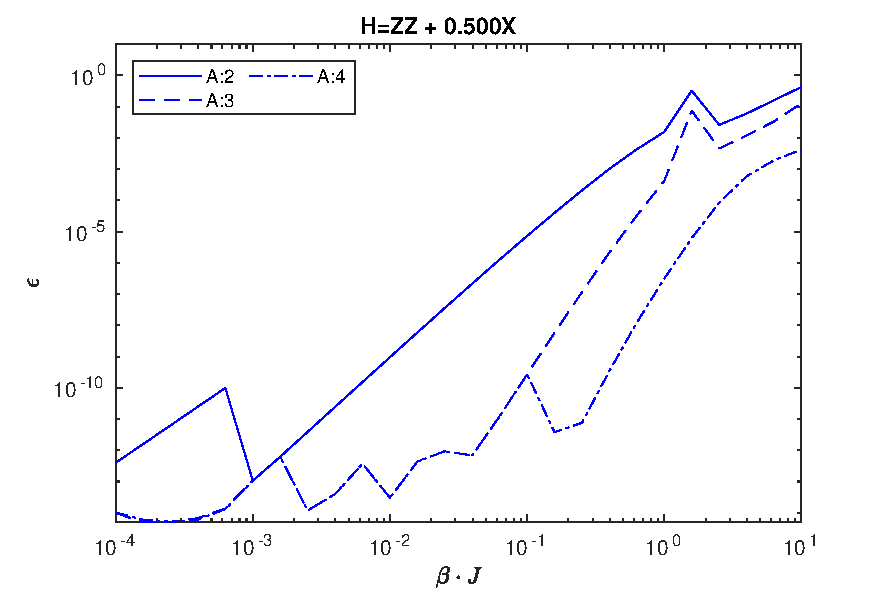
\includegraphics[width=0.8\linewidth]{Figuren/mpo_construction/sigm0/e11.pdf}
        \caption{${10}^{-11}$}
        \label{fig:sub2}
    \end{subfigure}
    \caption{A figure with two subfigures}
    \label{fig:sigman0}
\end{figure}

\begin{figure} \ContinuedFloat
    \centering
    \begin{subfigure}{\textwidth}
        \centering
        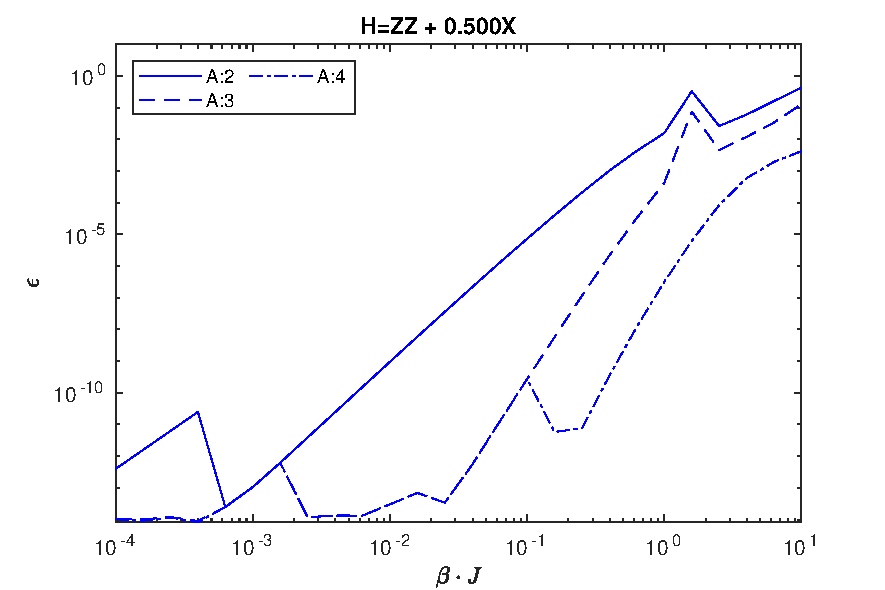
\includegraphics[width=0.8\linewidth]{Figuren/mpo_construction/sigm0/e12.pdf}
        \caption{ ${10}^{-12}$}
        \label{fig:sub1}
    \end{subfigure}%

    \begin{subfigure}{\textwidth}
        \centering
        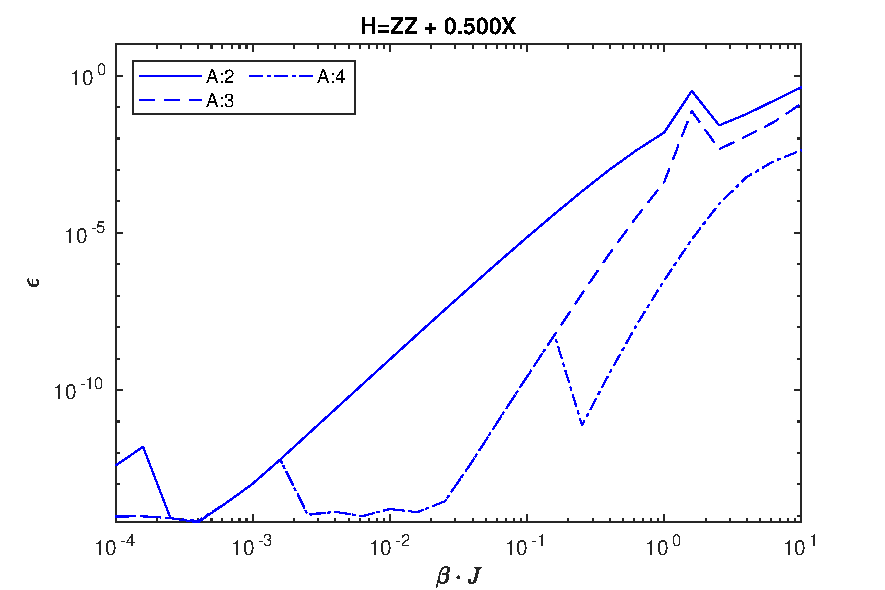
\includegraphics[width=0.8\linewidth]{Figuren/mpo_construction/sigm0/e13.pdf}
        \caption{${10}^{-13}$}
        \label{fig:sub2}
    \end{subfigure}
    \caption{A figure with two subfigures}
    \label{fig:sigman0}
\end{figure}

\begin{figure} \ContinuedFloat
    \centering
    \begin{subfigure}{\textwidth}
        \centering
        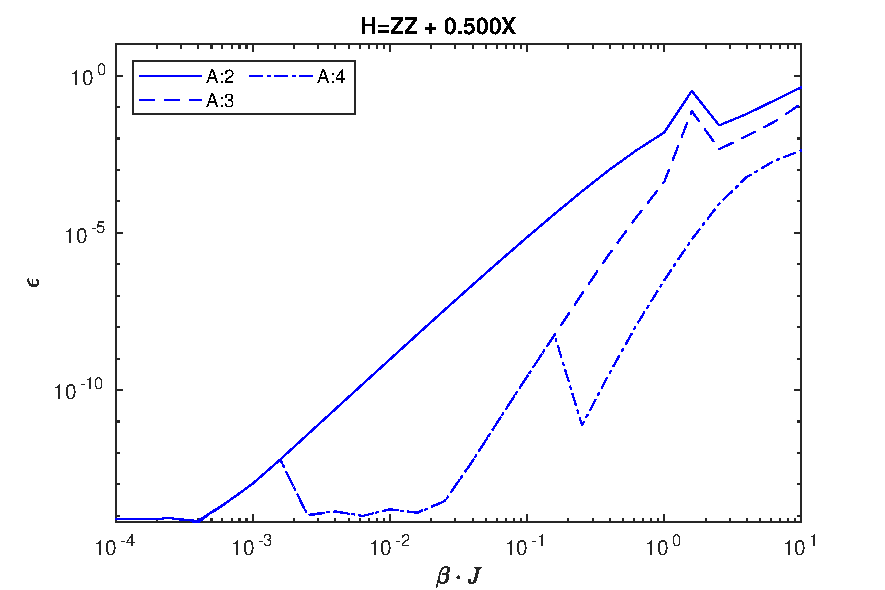
\includegraphics[width=0.8\linewidth]{Figuren/mpo_construction/sigm0/e14.pdf}
        \caption{ ${10}^{-14}$}
        \label{fig:sub1}
    \end{subfigure}%
    \caption{A figure with two subfigures}
    \label{fig:sigman0}
\end{figure}

In practice, the truncation criterium is not completely optimal in some specific cases.

\subsubsection{Type B}

Type B only contains blocks of the following form; $O^{m n}$ and $O^{n 0}$

\def \rhs{\expH{2}{ $L_{m}^{-1}  M_{n+1} $ }{{"$i_n$","$i_{n+1}$"}}{{"$j_n$","$j_{n+1}$"}}{{"m","0"}}  }
\begin{equation}
    \begin{split}
        \mpo{2}{ {"m","n","0"}  }{ { "$i_n$","$i_{n+1}$"}}{ { "$j_n$","$j_{n+1}$"}}{}{} &= \rhs \\
        &\cong X_{(\alpha_m i_n j_n)(i_{n+1} j_{n+1})}\\
        &= U^n  \Sigma V^{\dagger}
    \end{split}
\end{equation}

The following split is made: $O^{m n} \cong U^n$ and $O^{n 0} \cong  \Sigma V^{\dagger}$. In this way the inverse exists and doesn't need any calculation: $O^{m n} = U^{\dagger}$. \todo{implement this!}

\paragraph{dimension} From the construction the bond dimension grows from the left to the right. For the last step, there are only $d^2$ non zero singular values.  Each steps adds $d^2$ to the dimension.
For the last step, only $d^2$ non zero singular values need to be keeped. With the following natation:
\begin{equation}
    \begin{split}
        \mpo{1}{ {"m","n"}  }{ { "\(i\)",}}{ { "$j$",}}{}{} &= A^m_{ (\alpha i j ) \beta} \\
        \mpo{1}{ {"n","0"}  }{ { "$i$",}}{ { "$j$",}}{}{} &= B^n_{ (\alpha i j ) \beta} \\
    \end{split}
\end{equation}
The bond dimension of lower virtual levels can be reduced if we can solve the following equations simultaneously:

Then the MPO doesn't change if there are matrices $A'^{n}$, $A'^{n+1}$ and $B'^{n}$ such that
\begin{equation}
    \begin{split}
        S=A^{m} A^{n} &= A'^{m} A'^{n} \\
        T=A^{m} B^{n} &= A'^{m} B'^{n} \\
    \end{split}
\end{equation}
Such matrices with optimal bond dimension can be found with generalised SVD. Generalised SVD decomposes 2 matrices as follows:
\begin{equation}
    \begin{split}
        S^{\dagger} = (U \Sigma_1) Q^{\dagger} \\
        T^{\dagger} = (V \Sigma_2) Q^{\dagger}
    \end{split}
\end{equation}
The new bond dimension is the $\dim{n'} =d^2 \cdot \min( \dim{n-1}, \dim (n+1) )$.  The dimension is higher than type A.

\todo{meer uitleg gsvd https://nl.mathworks.com/help/matlab/ref/gsvd.html}

\paragraph{discussion}

This type has no parameters to fine tune. The only blocks appearing in this series expansion are explicitly calculated to lower the remaining error. The inverse is well defined. It is expected that the error increases strictly with increasing temperature and keeps decreasing for higher orders.

\subsubsection{Type C}
\todo{primed virtual levels}

This type implements the same strict type as Type B, blubut in a different way. No calculation is involved, except the calculation of the the exponentiated hamiltonian to certain order. The following kind of MPO strings are allowed:

\mpo{2}{{"0","1","0"}}{}{}{}{}
\mpo{3}{{"0","1'","2'","0"}}{}{}{}{}
\mpo{3}{{"0","1''","2''","0"}}{}{}{}{}
and so forth. All but one MPO elements are chosen to be the identity matrix. The middle one is the exponentiated hamiltonian with reshaped legs.

Primed levels are in fact just non overlapping virtual levels. They can be mapped to normal virtual levels.

\paragraph{discussion}
As can be expected from the construction, the bond dimension grows very fast. This type is just as precise as Type B.

\subsubsection{Type D}

This type uses a differemt setup which tries to capture the best of both Type A and B. Type  could handle long range correlation better because of the introuction of $O^{n n}$, but the inverse was not necesarily well defined. Type B had well conditioned inverses, but performed in most of the cases worse. The block appearing in type D are as follows:

\mpo{3}{{"m","n","n","m"}}{{,"-",}}{{,"-",}}{}{{"O","$D_n$","O"}} and \mpo{1}{{"n","n"}}{}{}{}{}

Similar to type A,

\def \rhs{\expH{2}{ $L_{n}^{-1}  M_{2n+2}  R_{n}^{-1}$ }{}{}{{"n","n"}}  }
\begin{equation}
    \begin{split}
        \mpo{3}{{"m","n","n","m"}}{{,"-",}}{{,"-",}}{}{{"O","$D_n$","O"}} &= \rhs \\
        &= U \Sigma V^{ \dagger}
    \end{split}
    \label{eq_nmn_level}
\end{equation}

Matrix $D_n$ is the singular value diagonal matrix devided by a normalisation factor $\phi$. Both U and V are multiplied by $  \sqrt{\phi} $.

\paragraph{discussion}
It's not completely clear what the values of $\phi$ should be.  If $\phi$ is to large, large chains are not surpressed. If phi is to small, the $O^{n n}$ blocks will become large and hence the chain will diverge again. A reasonable value is the sum of the singular values. \todo{other things could be tried here, WIP}

\paragraph{matrisation}
The cost of this type lies in the fact that it has no compact way of casting it to a matrix. The following works, but has quite a large dimension:

\begin{tabular}{ccc|cc|cc|cc}
    $O_{00}$               & $O_{01} $   &             & $-2  O_{01}$ &                & $ O_{01}$ &             & $ O_{01}  D_1^{1/2}$           &                                \\
    ${O_{10}}$             &             & ${ O_{12}}$ &              & $-2 { O_{12}}$ &           & ${ O_{12}}$ &                                &                                \\
                           & ${ O_{21}}$ &             &              &                &           &             &                                &                                \\
    \hline
    ${O_{10}}$             &             &             &              &                &           &             &                                &                                \\
                           & ${ O_{21}}$ &             &              &                &           &             &                                &                                \\
    \hline
    ${ O_{10}}$            &             &             &              &                & $O_{11}$  &             &                                &                                \\
                           & ${ O_{21}}$ &             &              &                &           & $O_{22}$    &                                &                                \\
    \hline
    $ D_1^{1/2} { O_{10}}$ &             &             &              &                &           &             &                                & $D_1^{-1/2} O_{12}  D_2^{1/2}$ \\
                           &             &             &              &                &           &             & $ D_2^{1/2} O_{21} D_1^{-1/2}$                                  \\\end{tabular}

\todo{fix this }

